% Fase 4: fundamentacao FAIR — fontes: monografia, cap. 6 (secoes 6.0.1--6.0.5).
% Diagramas TikZ originais e esquematicos. Nao representam resultados experimentais.
\setlength{\parskip}{3.5pt}
\definecolor{fairwarm}{RGB}{169,99,57}
\definecolor{fairref}{RGB}{128,144,153}
\newcommand{\FairAxes}{%
 \draw[->,gray!75] (-.12,0)--(6.25,0) node[below left,font=\scriptsize]{$f_1$};
 \draw[->,gray!75] (0,-.12)--(0,5.05) node[above left,font=\scriptsize]{$f_2$};}
\newcommand{\FairCurve}{\draw[very thick,fairref] plot[smooth] coordinates{(.8,4.35)(1.65,3.20)(2.65,2.38)(3.75,1.60)(5.45,.85)};}
\newcommand{\FairPt}[2]{\fill[fairwarm] (#1,#2) circle (3.1pt);}
\newcommand{\FairRefPt}[2]{\fill[fairref] (#1,#2) circle (2.0pt);}
\newcommand{\FairLegend}{\tikz[baseline=-.4ex]{\fill[fairref] (0,0) circle (2pt);}\,\scriptsize referência $R$\hspace{.6cm}\tikz[baseline=-.4ex]{\fill[fairwarm] (0,0) circle (2.7pt);}\,\scriptsize aproximação $P$}

\begin{frame}[plain]
\vspace*{2.0cm}
{\LARGE\color{navy}Métricas FAIR\par}
\vspace{.22cm}
{\large Caracterização estrutural de aproximações finitas\par}
{\large da frente de Pareto\par}
\vspace{.30cm}
\textcolor{navy!40}{\rule{.76\linewidth}{.65pt}}\par
\vspace{.20cm}
Medidas físicas e Q-scores calibrados.
\end{frame}

\begin{frame}{O que queremos conhecer sobre a frente resultante?}
Duas aproximações podem estar muito próximas da frente ótima, mas oferecer \textbf{conjuntos de alternativas bastante diferentes} para a tomada de decisão.
\begin{columns}[T,onlytextwidth]
\begin{column}{.49\textwidth}\centering
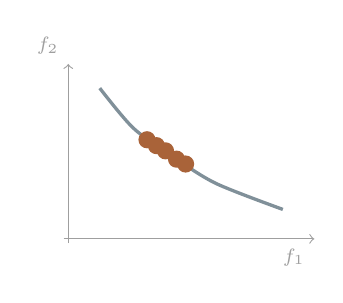
\begin{tikzpicture}[x=.50cm,y=.44cm]
\FairAxes\FairCurve
\foreach \x/\y in {2.0/2.86,2.24/2.69,2.47/2.54,2.75/2.30,2.98/2.16}{\FairPt{\x}{\y}}
\end{tikzpicture}
\textbf{A: soluções concentradas}\par
\scriptsize Pontos próximos da referência, mas restritos a uma pequena região.
\end{column}
\begin{column}{.49\textwidth}\centering
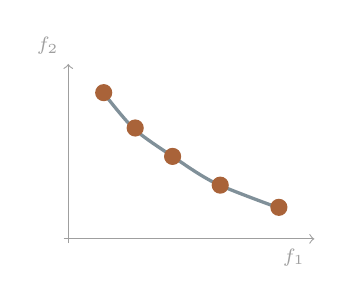
\begin{tikzpicture}[x=.50cm,y=.44cm]
\FairAxes\FairCurve
\foreach \x/\y in {.90/4.22,1.70/3.20,2.65/2.38,3.86/1.55,5.35/.91}{\FairPt{\x}{\y}}
\end{tikzpicture}
\textbf{B: soluções espalhadas}\par
\scriptsize A mesma ordem de proximidade, com opções em diferentes compromissos.
\end{column}
\end{columns}
\vspace{.16cm}
\textbf{Questão científica:} além da distância à frente ótima, como caracterizar \emph{cobertura, lacunas e organização espacial} das soluções?
\par{\scriptsize Diagramas esquemáticos de minimização; não são dados de um MOEA.}
\end{frame}

\begin{frame}{Por que não basta um único indicador agregado?}
O hypervolume resume a região dominada por uma aproximação. Esse número é útil para \textbf{comparar desempenho global}, mas não identifica, isoladamente, a natureza de cada deficiência espacial.
\begin{columns}[T,onlytextwidth]
\begin{column}{.47\textwidth}
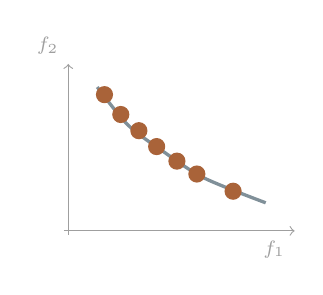
\begin{tikzpicture}[x=.46cm,y=.42cm]
\FairAxes\FairCurve
\foreach \x/\y in {1.0/4.12,1.45/3.52,1.95/3.03,2.44/2.55,3.00/2.11,3.55/1.72,4.55/1.20}{\FairPt{\x}{\y}}
\end{tikzpicture}
\textbf{Boa extensão, lacuna no extremo direito.}
\end{column}
\begin{column}{.51\textwidth}
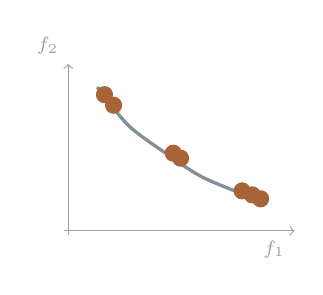
\begin{tikzpicture}[x=.46cm,y=.42cm]
\FairAxes\FairCurve
\foreach \x/\y in {1.0/4.12,1.25/3.80,2.9/2.35,3.10/2.20,4.80/1.21,5.08/1.09,5.31/.97}{\FairPt{\x}{\y}}
\end{tikzpicture}
\textbf{Boa extensão, mas agrupamentos e intervalos desiguais.}
\end{column}
\end{columns}
\vspace{.13cm}
\textbf{Proposta FAIR:} examinar propriedades distintas da aproximação, sem exigir que um único valor explique todas elas. Isso complementa HV, GD e IGD, sem substituí-los.
\end{frame}

\begin{frame}{Duas representações finitas: aproximação e referência}
\begin{columns}[T,onlytextwidth]
\begin{column}{.53\textwidth}
\begin{itemize}
\item $P=\{p_1,\ldots,p_K\}$: soluções não dominadas efetivamente examinadas.
\item $R=\{r_1,\ldots,r_N\}$: amostragem da frente de referência, denominada \emph{ground truth} (GT).
\item $d(x,S)=\min_{s\in S}\|x-s\|_2$: distância de um ponto ao elemento mais próximo de um conjunto.
\end{itemize}
\vspace{.12cm}
As direções \textbf{$P\to R$} e \textbf{$R\to P$} respondem a perguntas diferentes; a distância ao conjunto não é simétrica.
\end{column}
\begin{column}{.45\textwidth}\centering
\begin{tikzpicture}[x=.48cm,y=.49cm]
\FairAxes\FairCurve
\foreach \x/\y in {.8/4.35,1.5/3.4,2.2/2.74,2.9/2.2,3.6/1.69,4.3/1.35,5.45/.85}{\FairRefPt{\x}{\y}}
\FairPt{1.75}{3.68}\FairPt{2.5}{2.65}\FairPt{4.30}{1.63}
\draw[fairwarm,thick,->] (1.73,3.60)--(1.60,3.46);
\draw[navy,dashed,->] (3.55,1.70)--(2.56,2.60);
\node[font=\scriptsize,fairwarm] at (2.45,4.12) {$P\to R$};
\node[font=\scriptsize,navy] at (4.35,2.55) {$R\to P$};
\end{tikzpicture}
\FairLegend
\end{column}
\end{columns}
\end{frame}

\begin{frame}{Resolução finita: a cardinalidade $K$ estabelece uma escala}
Uma frente contínua precisa ser representada por um número finito de pontos. Mesmo uma aproximação \textbf{sobre a frente} deixa intervalos sem amostragem.
\begin{columns}[T,onlytextwidth]
\begin{column}{.55\textwidth}
\textbf{Uniform-at-$K$.} Selecionamos $U_K\subseteq R$ com $K$ pontos usando \emph{farthest point sampling} (FPS): cada novo ponto procura se afastar dos já selecionados.
\[
 s_K=\operatorname{med}_{u\in U_K}
 \min_{\substack{v\in U_K\\v\neq u}}\|u-v\|_2 .
\]
$s_K$ é o espaçamento típico de uma seleção bem distribuída com a \textbf{mesma cardinalidade}.
\end{column}
\begin{column}{.43\textwidth}\centering
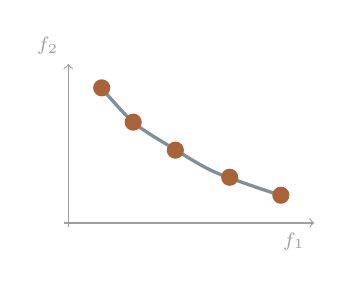
\begin{tikzpicture}[x=.50cm,y=.40cm]
\FairAxes\FairCurve
\foreach \x/\y in {.85/4.29,1.65/3.20,2.72/2.31,4.1/1.45,5.4/.88}{\FairPt{\x}{\y}}
\end{tikzpicture}
\textbf{$K=5$:} um conjunto bem distribuído ainda apresenta intervalos expressivos.
\end{column}
\end{columns}
\vspace{.12cm}
{\scriptsize Esquema didático: na implementação, FPS seleciona pontos da referência discreta $R$.}
\end{frame}

\begin{frame}{Mesma frente, mais pontos: resolução espacial mais fina}
\textbf{Por exemplo:} suponha que o mesmo GT seja representado por aproximações bem distribuídas com 5 ou com 9 pontos.
\begin{columns}[T,onlytextwidth]
\begin{column}{.49\textwidth}\centering
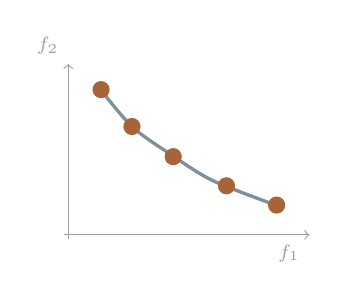
\begin{tikzpicture}[x=.49cm,y=.43cm]
\FairAxes\FairCurve
\foreach \x/\y in {.85/4.29,1.65/3.20,2.72/2.31,4.1/1.45,5.4/.88}{\FairPt{\x}{\y}}
\end{tikzpicture}
\textbf{$K=5$}: menor resolução.
\end{column}
\begin{column}{.49\textwidth}\centering
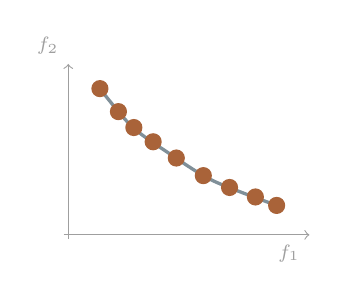
\begin{tikzpicture}[x=.49cm,y=.43cm]
\FairAxes\FairCurve
\foreach \x/\y in {.82/4.32,1.30/3.64,1.70/3.17,2.2/2.75,2.8/2.27,3.5/1.75,4.18/1.40,4.85/1.12,5.40/.87}{\FairPt{\x}{\y}}
\end{tikzpicture}
\textbf{$K=9$}: maior resolução.
\end{column}
\end{columns}
\vspace{.22cm}
\textbf{Consequência:} uma distância grande para $K=5$ pode ser compatível com a resolução disponível, mas indicar deficiência em $K=9$. É por isso que o protocolo considera $K$ ao calibrar os indicadores.
\end{frame}

\begin{frame}{Seis perguntas complementares sobre a aproximação}
\renewcommand{\arraystretch}{1.10}
\begin{tabularx}{\linewidth}{@{}>{\bfseries}p{.20\linewidth}X>{\raggedright\arraybackslash}p{.24\linewidth}@{}}
Closeness & Quão próximos da referência estão os pontos obtidos? & Distâncias $P\to R$\\
Coverage & Quanto da referência é representado por soluções próximas? & Distâncias $R\to P$\\
Gap & Existem regiões da referência particularmente mal cobertas? & Cauda de $R\to P$\\
Regularity & Os intervalos entre soluções seguem um padrão uniforme? & Vizinhos próximos\\
Balance & As soluções ocupam as regiões nas proporções esperadas? & Ocupação regional\\
Headway & Quanto do erro inicial da busca ainda permanece? & Inicial versus final\\
\end{tabularx}
\vspace{.04cm}
\textbf{Primeira camada:} todas as métricas físicas são orientadas a \textbf{minimização}: valores menores indicam menor discrepância segundo a propriedade considerada. Suas unidades não são necessariamente comparáveis.
\end{frame}

\begin{frame}{Closeness: as soluções alcançaram a frente?}
\textbf{Pergunta:} considerando cada solução obtida, a qual distância fica seu ponto de referência mais próximo?
\begin{columns}[T,onlytextwidth]
\begin{column}{.54\textwidth}
\[
\boxed{\displaystyle
C(P,R)=\max\!\left\{0,\;
\operatorname{med}_{p\in P}\frac{d(p,R)}{s_K}-\varepsilon_{\mathrm{ideal}}\right\}}
\]
\textbf{Mediana:} poucos pontos ruins não determinam sozinhos a proximidade típica.
\par\medskip
\textbf{$\varepsilon_{\mathrm{ideal}}$:} resíduo de discretização da referência previsto na calibração. Se nulo, resta a mediana das distâncias normalizadas.
\end{column}
\begin{column}{.44\textwidth}\centering
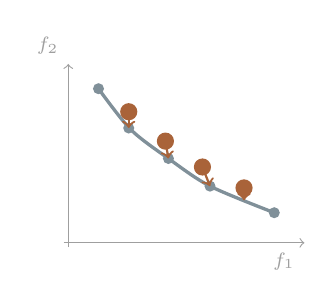
\begin{tikzpicture}[x=.48cm,y=.45cm]
\FairAxes\FairCurve
\foreach \x/\y in {.8/4.35,1.6/3.24,2.65/2.38,3.75/1.6,5.45/.85}{\FairRefPt{\x}{\y}}
\foreach \x/\y in {1.6/3.7,2.57/2.87,3.55/2.14,4.65/1.55}{\FairPt{\x}{\y}}
\foreach \a/\b/\c/\d in {1.6/3.7/1.6/3.24,2.57/2.87/2.65/2.38,3.55/2.14/3.75/1.6,4.65/1.55/4.65/1.2}{\draw[->,fairwarm,thick] (\a,\b)--(\c,\d);}
\end{tikzpicture}
\FairLegend
\end{column}
\end{columns}
\vspace{.08cm}\textbf{Interpretação:} valores baixos indicam aderência geométrica. Porém, um agrupamento de soluções sobre uma pequena região pode ter boa closeness e cobertura deficiente.
\end{frame}

\begin{frame}{Coverage: quais regiões da referência estão representadas?}
\textbf{Pergunta:} para cada ponto do GT, qual a distância até a solução produzida mais próxima?
\begin{columns}[T,onlytextwidth]
\begin{column}{.49\textwidth}
\[
\boxed{\displaystyle V(P,R)=\frac1{|R|}\sum_{r\in R}d(r,P)}
\]
\textbf{Contraste:} closeness examina $P\to R$, enquanto coverage examina $R\to P$.
\par\smallskip
Uma frente concentrada sobre um trecho do GT pode ter excelente proximidade, mas \textbf{não representar os outros trechos}.
\end{column}
\begin{column}{.49\textwidth}\centering
\begin{tikzpicture}[x=.46cm,y=.40cm]
\FairAxes\FairCurve
\foreach \x/\y in {.82/4.33,1.45/3.48,2.1/2.83,2.8/2.29,3.5/1.8,4.22/1.37,4.90/1.08,5.45/.85}{\FairRefPt{\x}{\y}}
\foreach \x/\y in {2.1/2.86,2.34/2.64,2.8/2.31,3.05/2.10}{\FairPt{\x}{\y}}
\draw[->,navy,thick] (.86,4.26)--(2.06,2.91);
\draw[->,navy,thick] (5.42,.91)--(3.12,2.07);
\end{tikzpicture}
\FairLegend
\end{column}
\end{columns}
\vspace{.13cm}
\textbf{Limitação:} o valor da média depende da amostragem de $R$: áreas representadas por mais pontos do GT recebem maior peso.
\end{frame}

\begin{frame}{Gap: qual é o tamanho dos afastamentos elevados?}
Coverage resume a \textbf{média} das distâncias $R\to P$. Isso pode ocultar regiões particularmente mal representadas.
\begin{columns}[T,onlytextwidth]
\begin{column}{.47\textwidth}
\[
\boxed{\displaystyle
G(P,R)=\operatorname{P}_{95}\{d(r,P):r\in R\}}
\]
\textbf{Pergunta:} até que distância vai a cauda superior das regiões menos bem representadas?
\par\medskip
\textbf{Intuição:} um único intervalo muito grande entre grupos de soluções pode exigir atenção, mesmo quando a média global parece aceitável.
\end{column}
\begin{column}{.51\textwidth}\centering
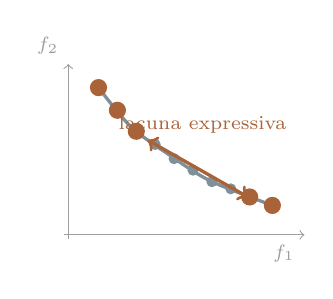
\begin{tikzpicture}[x=.48cm,y=.43cm]
\FairAxes\FairCurve
\foreach \x/\y in {.8/4.35,1.3/3.68,1.8/3.06,2.3/2.67,2.8/2.25,3.3/1.91,3.8/1.57,4.3/1.36,4.8/1.12,5.4/.87}{\FairRefPt{\x}{\y}}
\foreach \x/\y in {.8/4.35,1.3/3.68,1.8/3.06,4.8/1.12,5.4/.87}{\FairPt{\x}{\y}}
\draw[fairwarm,very thick,<->] (2.1,2.8)--(4.75,1.12);
\node[fairwarm,font=\scriptsize] at (3.55,3.25){lacuna expressiva};
\end{tikzpicture}
\FairLegend
\end{column}
\end{columns}
\vspace{.10cm}\textbf{Coverage versus gap:} a primeira pergunta quão bem coberta está a referência em média; a segunda destaca afastamentos grandes (percentil 95), sem depender do pior ponto isolado.
\end{frame}

\begin{frame}{Regularity: como estão espaçadas as soluções vizinhas?}
\textbf{Pergunta:} a aproximação apresenta o padrão de espaçamento local esperado para $K$ pontos distribuídos sobre a frente?
\begin{columns}[T,onlytextwidth]
\begin{column}{.54\textwidth}
\[
\boxed{\displaystyle
\operatorname{Reg}(P,R)=W_1\bigl(NN(P),NN(U_K)\bigr)}
\]
$NN(S)$ é a distribuição das distâncias ao vizinho mais próximo; $W_1$ mede a diferença entre as \textbf{distribuições de espaçamento}.
\par\medskip
$U_K$ é o padrão de comparação: $K$ pontos distribuídos sobre o GT por FPS.
\end{column}
\begin{column}{.44\textwidth}\centering
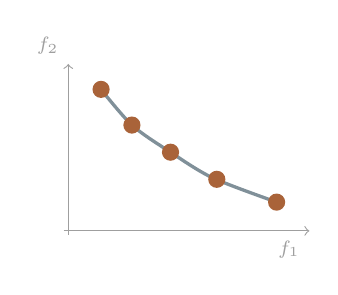
\begin{tikzpicture}[x=.49cm,y=.42cm]
\FairAxes\FairCurve
\foreach \x/\y in {.85/4.28,1.65/3.20,2.65/2.38,3.85/1.56,5.40/.87}{\FairPt{\x}{\y}}
\end{tikzpicture}
\textbf{Espaçamentos homogêneos}
\end{column}
\end{columns}
\vspace{.17cm}
\textbf{Interpretação:} regularity baixa indica que a distribuição de intervalos entre soluções se parece com a de $U_K$.
\end{frame}

\begin{frame}{Regularity e coverage não respondem à mesma pergunta}
\begin{columns}[T,onlytextwidth]
\begin{column}{.49\textwidth}\centering
\textbf{Espaçamento relativamente uniforme}\par\smallskip
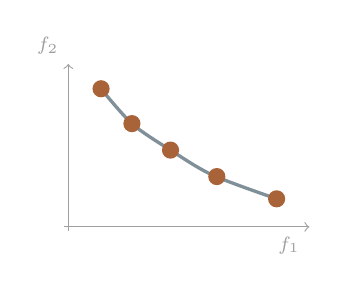
\begin{tikzpicture}[x=.49cm,y=.41cm]
\FairAxes\FairCurve
\foreach \x/\y in {.85/4.28,1.65/3.20,2.65/2.38,3.85/1.56,5.40/.87}{\FairPt{\x}{\y}}
\end{tikzpicture}
\end{column}
\begin{column}{.49\textwidth}\centering
\textbf{Pares próximos e intervalos grandes}\par\smallskip
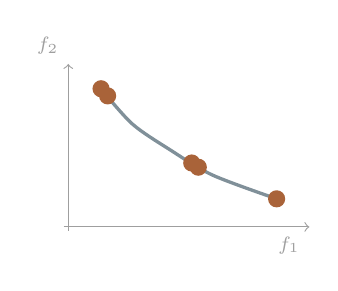
\begin{tikzpicture}[x=.49cm,y=.41cm]
\FairAxes\FairCurve
\foreach \x/\y in {.85/4.28,1.02/4.06,3.20/1.98,3.37/1.85,5.4/.87}{\FairPt{\x}{\y}}
\end{tikzpicture}
\end{column}
\end{columns}
\vspace{.14cm}
\textbf{Por exemplo:} ambos os conjuntos atingem os extremos da frente, mas o segundo agrupa soluções em pares e deixa grandes intervalos entre eles.
\par\medskip
\textbf{Contraste:} coverage mede a distância média do GT às soluções; regularity mede \emph{como os intervalos entre soluções estão distribuídos}. Uma não substitui a outra.
\end{frame}

\begin{frame}{Balance: quantos pontos há em cada região?}
\textbf{Pergunta:} os pontos produzidos ocupam as regiões do GT em proporções semelhantes às de uma seleção uniforme de $K$ pontos?
\begin{columns}[T,onlytextwidth]
\begin{column}{.51\textwidth}
\[
\boxed{\displaystyle
B(P,R)=\sqrt{D_{\mathrm{JS}}(H_P\parallel H_{U_K})}}
\]
Os centróides definidos sobre $R$ delimitam regiões de ocupação. $H_P$ e $H_{U_K}$ são histogramas normalizados das proporções de pontos atribuídas a essas regiões.
\par\medskip
\textbf{Regularity versus balance:} regularity avalia distâncias locais entre vizinhos; balance compara o \emph{peso relativo de cada região}.
\end{column}
\begin{column}{.47\textwidth}\centering
\textbf{Distribuição regional de 10 soluções}\par\medskip
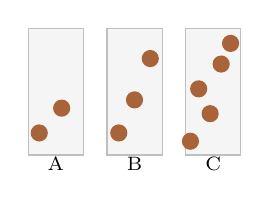
\begin{tikzpicture}[x=.50cm,y=.35cm]
\foreach \x/\n/\m in {0/2/5,2/3/5,4/5/5}{
\draw[fill=gray!8,draw=gray!50] (\x,0) rectangle +(1.4,4.6);
\node[font=\scriptsize] at (\x+.7,-.32) {\ifnum\x=0 A\else\ifnum\x=2 B\else C\fi\fi};}
\foreach \x/\y in {.28/.8,.85/1.7,2.3/.8,2.7/2.0,3.1/3.5,4.12/.5,4.62/1.5,4.33/2.4,4.9/3.3,5.14/4.05}{\FairPt{\x}{\y}}
\end{tikzpicture}
\scriptsize Exemplo esquemático: A recebe 2 pontos, B recebe 3, C recebe 5. O equilíbrio depende das proporções no baseline $U_K$.
\end{column}
\end{columns}
\vspace{.06cm}\textbf{Interpretação:} baixa distância indica proporções regionais semelhantes às do padrão de referência, não necessariamente distância pequena ao GT.
\end{frame}

\begin{frame}{Headway: a busca melhorou em relação ao ponto de partida?}
\textbf{Pergunta:} que fração do afastamento inicial ainda permanece ao terminar o MOEA?
\[
\boxed{\displaystyle H=\frac{GD_{95}(P_{\mathrm{final}}\to R)}{GD_{95}(P_{\mathrm{inicial}}\to R)}}
\]
$GD_{95}$ é o percentil 95 das distâncias $P\to R$. Ao contrário de closeness, headway usa \textbf{duas populações de uma mesma execução}.
\begin{columns}[T,onlytextwidth]
\begin{column}{.49\textwidth}
\textbf{$H=0{,}16$} significa que restaram 16\% do erro inicial, isto é, houve redução de aproximadamente \textbf{84\%} no indicador longitudinal.
\end{column}
\begin{column}{.49\textwidth}
\textbf{$H\approx1$} indica pouca redução; $H>1$ indica aumento do afastamento. É uma \textbf{razão}, não uma medida de proximidade final.
\end{column}
\end{columns}
\vspace{.17cm}
A interpretação requer cautela quando o denominador inicial é muito pequeno: uma população já próxima da frente oferece pouca margem para melhora relativa.
\end{frame}

\begin{frame}{Closeness e headway: resultado final versus progresso}
Duas execuções terminam com \textbf{erro final igual}, $GD_{95}=0{,}4$, mas partem de condições diferentes (valores ilustrativos).
\begin{columns}[T,onlytextwidth]
\begin{column}{.49\textwidth}\centering
\textbf{Execução A}\par\vspace{.02cm}
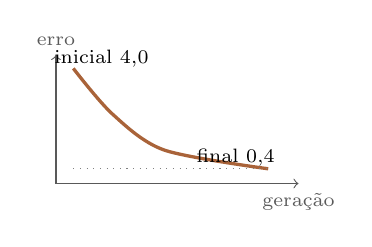
\begin{tikzpicture}[x=.55cm,y=.34cm]
\draw[->,black!65] (0,0)--(5.6,0) node[below,font=\scriptsize]{geração};
\draw[->,black!65] (0,0)--(0,4.8) node[above,font=\scriptsize]{erro};
\draw[very thick,fairwarm] plot[smooth] coordinates{(.4,4.3)(1.3,2.6)(2.5,1.25)(4.9,.55)};
\draw[dotted,gray] (.4,.55)--(4.9,.55);
\node[font=\scriptsize] at (1.05,4.65){inicial $4{,}0$};
\node[font=\scriptsize] at (4.15,.95){final $0{,}4$};
\end{tikzpicture}
\[ H_A=0{,}4/4{,}0=0{,}10 \]
Grande redução durante a busca.
\end{column}
\begin{column}{.49\textwidth}\centering
\textbf{Execução B}\par\vspace{.02cm}
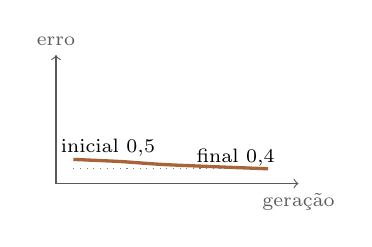
\begin{tikzpicture}[x=.55cm,y=.34cm]
\draw[->,black!65] (0,0)--(5.6,0) node[below,font=\scriptsize]{geração};
\draw[->,black!65] (0,0)--(0,4.8) node[above,font=\scriptsize]{erro};
\draw[very thick,fairwarm] plot[smooth] coordinates{(.4,.90)(1.5,.82)(2.6,.70)(4.9,.55)};
\draw[dotted,gray] (.4,.55)--(4.9,.55);
\node[font=\scriptsize] at (1.2,1.35){inicial $0{,}5$};
\node[font=\scriptsize] at (4.15,.95){final $0{,}4$};
\end{tikzpicture}
\[ H_B=0{,}4/0{,}5=0{,}80 \]
A população já começou próxima.
\end{column}
\end{columns}
\textbf{Interpretação:} B já começou perto do GT, possivelmente por sorte. A boa proximidade final não significa que o MOEA tenha progredido muito. Headway destaca isso, sem provar a causa.
\end{frame}

\begin{frame}{Medidas físicas: seis dimensões, réguas diferentes}
\renewcommand{\arraystretch}{1.10}
\begin{tabularx}{\linewidth}{@{}>{\bfseries}p{.22\linewidth}p{.29\linewidth}X@{}}
Closeness & Distância em unidades de $s_K$ & Quanto menor, mais próximos os pontos produzidos.\\
Coverage, gap & Distância geométrica & Quanto menor, menores a média ou as grandes lacunas.\\
Regularity & Distância $W_1$ entre distribuições & Quanto menor, mais parecido o padrão de espaçamentos.\\
Balance & Distância entre distribuições regionais & Quanto menor, mais semelhante a distribuição por regiões.\\
Headway & Razão de erros & Quanto menor, maior a redução relativa de afastamento.\\
\end{tabularx}
\vspace{.08cm}
\textbf{Problema:} o que significaria comparar diretamente um gap de 0,15 a um headway de 0,15? As unidades, a geometria do MOP e o número de soluções são diferentes.
\par\smallskip
\textbf{Segunda camada:} calibrar cada medida contra condições favoráveis e desfavoráveis \emph{específicas da dimensão}, produzindo uma escala de apresentação comum.
\end{frame}

\begin{frame}{Calibração: quem define o que é favorável?}
A referência física e a cardinalidade efetiva $K$ permitem construir \textbf{padrões reproduzíveis} de desempenho, associados ao MOP e à sua resolução.
\begin{columns}[T,onlytextwidth]
\begin{column}{.49\textwidth}\centering
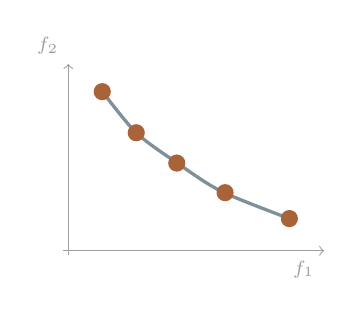
\begin{tikzpicture}[x=.52cm,y=.47cm]
\FairAxes\FairCurve
\foreach \x/\y in {.83/4.30,1.66/3.19,2.65/2.37,3.83/1.57,5.40/.87}{\FairPt{\x}{\y}}
\end{tikzpicture}
\textbf{Favorável: Uniform-at-$K$}\par
\scriptsize FPS espalha $K$ pontos sobre o GT; estabelece a referência favorável para cobertura e distribuição.
\end{column}
\begin{column}{.49\textwidth}\centering
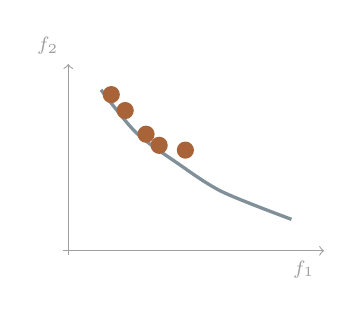
\begin{tikzpicture}[x=.52cm,y=.47cm]
\FairAxes\FairCurve
\foreach \x/\y in {1.05/4.22,1.39/3.79,1.9/3.15,2.22/2.85,2.86/2.72}{\FairPt{\x}{\y}}
\end{tikzpicture}
\textbf{Desfavorável: distribuição aleatória / perturbada}\par
\scriptsize Baselines são simulados conforme a propriedade, e não uma única população ``ruim'' universal.
\end{column}
\end{columns}
\vspace{.13cm}
Para \textbf{coverage, gap, regularity e balance}, a calibração armazena a mediana favorável (\texttt{uni50}), a mediana aleatória (\texttt{rand50}) e a distribuição empírica aleatória (\texttt{rand\_ecdf}).
\end{frame}

\begin{frame}{Q-score: a mesma escala, não a mesma grandeza}
Um \textbf{Q-score} traduz a posição de uma medida física entre os extremos do \emph{seu próprio protocolo de calibração}.
\begin{columns}[T,onlytextwidth]
\begin{column}{.55\textwidth}
\textbf{Para coverage, gap, regularity e balance:}
\[
\boxed{\displaystyle
Q(x)=1-\operatorname{clip}_{[0,1]}
\!\left(\frac{F_{\rm rand}(x)-F_{\rm rand}(x_{\rm ideal})}
{F_{\rm rand}(x_{\rm rand})-F_{\rm rand}(x_{\rm ideal})}\right)}
\]
$F_{\rm rand}$ é a distribuição acumulada empírica do baseline aleatório; $x_{\rm ideal}$ e $x_{\rm rand}$ são os referenciais favorável e desfavorável armazenados.
\end{column}
\begin{column}{.43\textwidth}\centering
\begin{tikzpicture}[x=.57cm,y=.58cm]
\draw[->] (0,0)--(5.6,0) node[below,font=\scriptsize]{$x$: erro físico};
\draw[->] (0,0)--(0,4.3) node[left,font=\scriptsize]{$F_{\rm rand}(x)$};
\draw[fairwarm,very thick] (0.5,.25)--(1.3,.25)--(1.3,.95)--(2.05,.95)--(2.05,1.65)--(2.8,1.65)--(2.8,2.4)--(3.6,2.4)--(3.6,3.15)--(4.45,3.15)--(4.45,3.85)--(5.1,3.85);
\draw[dashed,navy] (1.05,0)--(1.05,4);
\draw[dashed,navy] (3.75,0)--(3.75,4);
\node[font=\scriptsize,navy] at (1.05,-.45){ideal};
\node[font=\scriptsize,navy] at (3.75,-.45){rand};
\end{tikzpicture}
\scriptsize Esquema da CDF empírica, não dados reais.
\end{column}
\end{columns}
\vspace{.10cm}\textbf{$Q\approx1$:} próximo do padrão favorável; \textbf{$Q\approx0$:} próximo do desfavorável. Um Q-score de 0,8 \textbf{não} significa 80\% de cobertura da frente.
\end{frame}

\begin{frame}{Cada Q-score utiliza a sua própria calibração}
\textbf{Todas as dimensões compartilham a escala $[0,1]$, mas não compartilham a mesma medida física ou transformação.}
\vspace{.12cm}
\renewcommand{\arraystretch}{1.22}
\begin{tabularx}{\linewidth}{@{}>{\bfseries}p{.30\linewidth}X@{}}
Coverage, gap, regularity e balance & CDF empírica do baseline aleatório, referida a padrões Uniform-at-$K$ e aleatório.\\
Closeness & Perturbação positiva do GT com ruído \emph{Half-Normal} e comparação distribucional via Wasserstein.\\
Headway & Transformação log-linear da razão de erro entre a população final e a inicial.\\
\end{tabularx}
\vspace{.24cm}
\textbf{Conclusão:} um Q-score de 0,8 para coverage e outro de 0,8 para headway não são duas medidas de 80\% da mesma grandeza. Representam posições favoráveis \emph{dentro de duas calibrações distintas}.
\end{frame}

\begin{frame}{Como interpretar um perfil de Q-scores?}
\textbf{Perfil ilustrativo}, com seis escores calibrados em $[0,1]$; não corresponde a uma execução real.
\begin{columns}[T,onlytextwidth]
\begin{column}{.54\textwidth}
\renewcommand{\arraystretch}{1.05}
\begin{tabular}{@{}lrr@{}}
\textbf{Dimensão} & \textbf{Q-score} & \textbf{Leitura} \\
Closeness & $0{,}90$ & Favorável \\
Coverage & $0{,}25$ & Fraco \\
Gap & $0{,}10$ & Muito fraco \\
Regularity & $0{,}70$ & Razoável \\
Balance & $0{,}15$ & Fraco \\
Headway & $0{,}95$ & Favorável \\
\end{tabular}
\par\smallskip
\textbf{O perfil deve ser lido por dimensão, não pela média dos escores.}
\end{column}
\begin{column}{.43\textwidth}\centering
\begin{tikzpicture}[x=.40cm,y=.40cm]
\foreach \yy/\v in {6/9,5/2.5,4/1,3/7,2/1.5,1/9.5}{
 \draw[gray!30] (0,\yy) rectangle (10,\yy+.42);
 \fill[navy!72] (0,\yy) rectangle (\v,\yy+.42);
}
\node[below,font=\scriptsize] at (0,1){0};
\node[below,font=\scriptsize] at (10,1){1};
\end{tikzpicture}
\end{column}
\end{columns}
\vspace{.03cm}\textbf{Exemplo:} a frente ficou próxima do GT e houve progresso, mas há lacunas e desequilíbrio regional. Closeness e headway altos não apagam coverage, gap e balance baixos.
\end{frame}

\begin{frame}[fragile]{Do diagnóstico à investigação dos resultados}
\begin{columns}[T,onlytextwidth]
\begin{column}{.49\textwidth}
\begin{lstlisting}[style=python,basicstyle=\ttfamily\fontsize{7.8}{10}\selectfont]
diagnosis = mb.clinic.audit(exp)
diagnosis.report()

mb.view.radar(diagnosis)
mb.view.ecdf(exp, metric='closeness')
mb.view.history(exp,
   domain='clinic', metric='coverage')
\end{lstlisting}
\par\medskip
\textbf{Instrumentos distintos:} números físicos, escores calibrados, perfil multidimensional, distribuição de distâncias e evolução temporal.
\end{column}
\begin{column}{.48\textwidth}
\textbf{Perguntas para orientar a leitura}\par\smallskip
\begin{itemize}
\item \textbf{Onde foi bem?} Quais Q-scores se aproximam do baseline favorável?
\item \textbf{Onde foi mal?} O problema é proximidade, extensão, lacunas ou distribuição?
\item \textbf{Qual evidência confirma?} Como aparecem as distâncias, o histórico e a topologia?
\end{itemize}
\end{column}
\end{columns}
\vspace{.17cm}
\textbf{Próxima seção:} aplicar essa leitura a resultados reais de DTLZ e DPF, comparando perfis e comentando especificamente o que cada figura evidencia.
\end{frame}